\chapter{Measurements and results}
\section{General remarks}
A photoacoustic measurement requires a chopper to modulate the incoming laser at the longitudinal resonance frequency of the chamber, in order to maximize the signal measured by the microphones.

About the microphones, it should be noticed that we didn't know their gain, neither it was possible with our instruments to make a calibration curve. In addition, we thought that understanding in deep the complicated, though interesting, physical processes between the photon absorption and the acoustic wave generation was too far from the general purpose of this work. This implies that, throughout this report, the absorption magnitude signals won't be reported neither with the dimensions of gas absorbance neither with the mechanical dimensions of sound waves. Instead they will be reported in volts, that is, the true (amplified) microphone output that entered the lock-in amplifier. This choice, instead of just using arbitrary units, at least allows us to compare results from different measurements, or even compare our data with those from other groups that used our very same microphones.
\section{Finding chamber resonances}
The first step of the measurement session was dedicated to find the best resonant frequency. We were told about an approximated length of the internal chamber of 10 cm, hence we expected the first resonating longitudinal mode to be a $\simeq20$ cm long wave. Considering the chamber full of atmospheric pressure \ce{O2} at room temperature, with sound speed 326 m/s this corresponds to a frequency of 1630 Hz.

	\subsection{Open chamber measurement}
We did the measurement stimulating the air inside the chamber through a speaker connected to a waveform generator, and looking at the signal coming from microphones. Since we were not able to insert a speaker inside the chamber (this was small), we excited the open chamber from outside through a hole. The resulting spectrum is shown in \cref{chamberplot}.
\begin{figure}[!bht]\centering
% GNUPLOT: LaTeX picture with Postscript
\begingroup
  \makeatletter
  \providecommand\color[2][]{%
    \GenericError{(gnuplot) \space\space\space\@spaces}{%
      Package color not loaded in conjunction with
      terminal option `colourtext'%
    }{See the gnuplot documentation for explanation.%
    }{Either use 'blacktext' in gnuplot or load the package
      color.sty in LaTeX.}%
    \renewcommand\color[2][]{}%
  }%
  \providecommand\includegraphics[2][]{%
    \GenericError{(gnuplot) \space\space\space\@spaces}{%
      Package graphicx or graphics not loaded%
    }{See the gnuplot documentation for explanation.%
    }{The gnuplot epslatex terminal needs graphicx.sty or graphics.sty.}%
    \renewcommand\includegraphics[2][]{}%
  }%
  \providecommand\rotatebox[2]{#2}%
  \@ifundefined{ifGPcolor}{%
    \newif\ifGPcolor
    \GPcolorfalse
  }{}%
  \@ifundefined{ifGPblacktext}{%
    \newif\ifGPblacktext
    \GPblacktexttrue
  }{}%
  % define a \g@addto@macro without @ in the name:
  \let\gplgaddtomacro\g@addto@macro
  % define empty templates for all commands taking text:
  \gdef\gplbacktext{}%
  \gdef\gplfronttext{}%
  \makeatother
  \ifGPblacktext
    % no textcolor at all
    \def\colorrgb#1{}%
    \def\colorgray#1{}%
  \else
    % gray or color?
    \ifGPcolor
      \def\colorrgb#1{\color[rgb]{#1}}%
      \def\colorgray#1{\color[gray]{#1}}%
      \expandafter\def\csname LTw\endcsname{\color{white}}%
      \expandafter\def\csname LTb\endcsname{\color{black}}%
      \expandafter\def\csname LTa\endcsname{\color{black}}%
      \expandafter\def\csname LT0\endcsname{\color[rgb]{1,0,0}}%
      \expandafter\def\csname LT1\endcsname{\color[rgb]{0,1,0}}%
      \expandafter\def\csname LT2\endcsname{\color[rgb]{0,0,1}}%
      \expandafter\def\csname LT3\endcsname{\color[rgb]{1,0,1}}%
      \expandafter\def\csname LT4\endcsname{\color[rgb]{0,1,1}}%
      \expandafter\def\csname LT5\endcsname{\color[rgb]{1,1,0}}%
      \expandafter\def\csname LT6\endcsname{\color[rgb]{0,0,0}}%
      \expandafter\def\csname LT7\endcsname{\color[rgb]{1,0.3,0}}%
      \expandafter\def\csname LT8\endcsname{\color[rgb]{0.5,0.5,0.5}}%
    \else
      % gray
      \def\colorrgb#1{\color{black}}%
      \def\colorgray#1{\color[gray]{#1}}%
      \expandafter\def\csname LTw\endcsname{\color{white}}%
      \expandafter\def\csname LTb\endcsname{\color{black}}%
      \expandafter\def\csname LTa\endcsname{\color{black}}%
      \expandafter\def\csname LT0\endcsname{\color{black}}%
      \expandafter\def\csname LT1\endcsname{\color{black}}%
      \expandafter\def\csname LT2\endcsname{\color{black}}%
      \expandafter\def\csname LT3\endcsname{\color{black}}%
      \expandafter\def\csname LT4\endcsname{\color{black}}%
      \expandafter\def\csname LT5\endcsname{\color{black}}%
      \expandafter\def\csname LT6\endcsname{\color{black}}%
      \expandafter\def\csname LT7\endcsname{\color{black}}%
      \expandafter\def\csname LT8\endcsname{\color{black}}%
    \fi
  \fi
  \setlength{\unitlength}{0.0500bp}%
  \begin{picture}(7200.00,5040.00)%
    \gplgaddtomacro\gplbacktext{%
      \csname LTb\endcsname%
      \put(682,704){\makebox(0,0)[r]{\strut{} 0}}%
      \put(682,1112){\makebox(0,0)[r]{\strut{} 1}}%
      \put(682,1521){\makebox(0,0)[r]{\strut{} 2}}%
      \put(682,1929){\makebox(0,0)[r]{\strut{} 3}}%
      \put(682,2337){\makebox(0,0)[r]{\strut{} 4}}%
      \put(682,2746){\makebox(0,0)[r]{\strut{} 5}}%
      \put(682,3154){\makebox(0,0)[r]{\strut{} 6}}%
      \put(682,3562){\makebox(0,0)[r]{\strut{} 7}}%
      \put(682,3971){\makebox(0,0)[r]{\strut{} 8}}%
      \put(682,4379){\makebox(0,0)[r]{\strut{} 9}}%
      \put(814,484){\makebox(0,0){\strut{} 0}}%
      \put(2012,484){\makebox(0,0){\strut{} 2000}}%
      \put(3210,484){\makebox(0,0){\strut{} 4000}}%
      \put(4407,484){\makebox(0,0){\strut{} 6000}}%
      \put(5605,484){\makebox(0,0){\strut{} 8000}}%
      \put(6803,484){\makebox(0,0){\strut{} 10000}}%
      \put(176,2541){\rotatebox{-270}{\makebox(0,0){\strut{}Magnitude [arbitrary units]}}}%
      \put(3808,154){\makebox(0,0){\strut{}Frequency [Hz]}}%
      \put(3808,4709){\makebox(0,0){\strut{}Open chamber resonances spectrum}}%
      \put(1767,2460){\makebox(0,0){\strut{}1591 Hz}}%
    }%
    \gplgaddtomacro\gplfronttext{%
    }%
    \gplbacktext
    \put(0,0){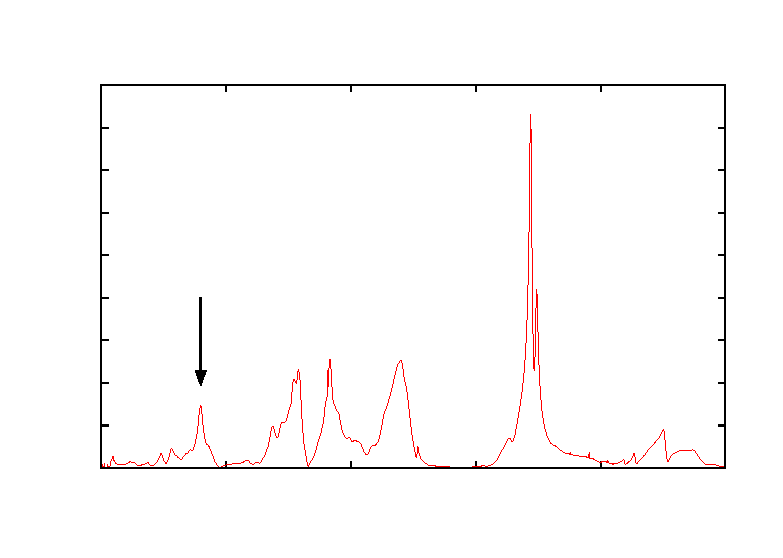
\includegraphics{chamber}}%
    \gplfronttext
  \end{picture}%
\endgroup

\caption{Spectrum of the open chamber, excited with a loudspeaker. The magnitude is set in arbitrary units because this spectrum has been acquired by a software whose unity conversion settings we couldn't control.}
\label{chamberplot}
\end{figure}
In doing this, we differ from the true experimental conditions in three aspects:
\begin{itemize}
\item we have air instead of \ce{O2}
\item we have an open chamber instead of a closed one 
\item the wave signal coming from a small hole aside, instead of being generated in the middle of the chamber.
\end{itemize}

In principle it's easy to correct the spectrum taken in air, in order to apply it to oxygen: in first approximation one has to deal just with a different sound velocity. On the other side, it is more difficult to take into account the acoustic and dynamic modifications the chamber undergoes for being open or closed, as well as for the pressure wave to be originated from a lateral point instead of a diffused volume within the chamber. For these reasons, this cannot be considered as a true spectrum for the chamber we actually used in the absorption measurement. It is nothing more than a useful starting point. Eventually the real resonance frequency had to be experimentally determined with a closed chamber full of oxygen excited from the laser. Also the frequency response of both the loudspeaker and the microphones were unknown, and this could in principle affect the shape of this plot. We looked in a range from 0 to 10 kHz, although we later observed that our chopper wouldn't be able to reach frequencies above few kHz.

We located a clear peak at 1591 Hz, which can attributed to the first longitudinal mode of the chamber, assuming a length $l$ of the chamber slighty greater than the declared 10 cm$$l=\frac{343\mbox{ m/s}}{1591\mbox{ Hz}}\cdot\frac{1}{2}=10.78\mbox{ cm}$$.

		\subsection{Closed chamber measurement}
Starting from the open chamber datum, we injected \ce{O2} in the chamber and started to look for signal by chopping the laser at 1591 Hz. It was promptly clear that there would not be need to further seek for resonances, as the intensity of the signal was high enough even at 1591 Hz, without any correction due to the gas change. We thus decided to delay the search for the acoustic resonance peak in oxygen and proceed with the experiment, in order to save time and give more attention to other issues such as stabilizing the laser emission or look for the oxygen absorption peaks.

Later, at the end of the experiment, we decided that completeness required us to provide the value of maximum resonance with oxygen, even though our measurement were all taken at 1591 Hz. Since the mechanical chopper failed to follow the waveform generator even for the slowest frequency sweep, we couldn't take a spectrum. Changing the frequency by hand we found however the peak at 1512 Hz, where we expected it according to a sound speed in atmospheric pressure oxygen of 323 m/s and a chamber length of 10.78 cm$$f^{\mai{peak}}_{\ce{o2}}=\frac{323\mbox{ m/s}}{2\cdot10.77\mbox{ cm}}\simeq1512\mbox{ Hz.}$$

\section{Looking for the \texorpdfstring{\ce{O2}}{} peaks (UNDER CONSTRUCTION)}
The next step after setting up and optimizing the apparatus was trying to find the best measurement conditions to see the peak. This means to find the frequency of the \ce{O2} absorption peaks, and some absorption peaks of the oxygen molecule trying the different acoustic resonance frequences and changing the laser parameters (current, temperature and position of our piezoelectric actuators). 
We were able to measure absorption at various different frequences. 

tabella MONOCOLONNA?? ? TABELLA!!! 

[[x ZENO: AGIGUNGIAMO UN CONFRONTO COI DATI DI HAAARP?]]

During this measurements we first noticed the instability of our laser emission in time. For example, when we found some peak at a certain injection current, 
temperature and piezoelectric position, after some minutes that peak would  "drift away"/[evolve?] and we needed to change the piezoelectric position in order to find it again.
After more time (a couple of hours) the peak would decrease in intensity and eventually fade completely, forcing us to change temperature or current of the laser
in order to see it again (or to find some other peak). We will discuss more accurately this uncontrolled frequency evolution effect in the next sections. 

\section{Shape of the peaks (UNDER CONSTRUCTION)}\label{shapeaks}
After having found some absorption peaks and approximately measured their wavelength using the spectrometer, we tried to acquire their shape as well. As seen in \cref{lasersource}, the piezoelectric tunability was too narrow to acquire one whole peak, so it was important to understand which section of the peak we were looking at. This information allowed us to acquire different points of the same absorption peak, by slightly modifying the output frequency of the laser. The frequency instability in time of the laser output was the biggest deal in doing these measurements. 

In order to find the best way to observe the peaks shape, we needed to control many parameters at the same time. Then we used a computer and a data acquisition board exploiting four analog inputs. In this way we were able to log:
\begin{itemize}
	\item the magnitude of the audio wave coming from the lock-in amplifier
	\item the position of the piezoelectric actuator responsible for the rotation of the grating around the $z$ axis
	\item the wavelength of the highest laser peak, roughly estimated with the spectroscope software, after having it converted to an analog signal through the integrated DAC
	\item the intensity of such peak or, depending on the needs, the ratio between the intensity of the peak and its integral (in order to detect multi-modal emission).
\end{itemize}
The measurements were performed by sweeping the position of the piezoelectric actuators with the waveform generator. 
The measurements we did using this setup can be divided in 3 categories: single full sweeps, multiple full sweeps and multiple focused sweeps. 
		\subsection{Single full sweeps} 
In this kind of measurement, we set the laser diode temperature and injection current, waited about 15 minutes to get emission stability, and started sweeping the piezoelectric crystal along its full driving range (0-150 V), using a linear ramp function with a period of about 11 minutes. This kind of experiment showed all the different absorption peaks available with that choice of laser parameters, and also to study the periodicity of the laser modes with respect to the grating position.

\medskip
\cref{primopicco,moltipicchi} show the result of this first session of measurements. In \cref{fullsweep1} a full sweep of the piezoelectric actuators made the laser to hop its emission mode many times. But only few of those modes met the absorption peak of the oxygen, thus resulting in a high signal. In \cref{fullsweep2} the same modes give a much lower signal: we moved far away from the absorption peak maximum.
MA WTF HAPPENED? MAGIC DRIFT DI COSA?
In \cref{moltipicchi} we slightly changed one of the laser parameters: the diode temperature. The whole modes pattern is now completely reshuffled with respect to \cref{primopicco}, and the full sweep of the piezoelectric actuators shown in \cref{bevified} now highlights three different absorption peaks. A closer observation, in \cref{magnified}, permits to fully appreciate this, as well as to see the signal deformation due to the lock-in integrator. 

\begin{figure}[!hptb]\centering
\subfigure[Absorption, maximum of a peak. Laser parameters: 29.16 $^\circ$C; 73.23 mA.\label{fullsweep1}]{\includegraphics[width=\linewidth, height=10cm, draft=\foto]{eps/Graph6.eps}} 
\subfigure[Absorption, tail of a peak. Laser parameters: 29.16 $^\circ$C; 73.23 mA.\label{fullsweep2}]{\includegraphics[width=\linewidth, height=10cm, draft=\foto]{eps/Graph7.eps}}
\caption{Photoacoustic absorption of a $\simeq$ 687.0 nm peak. The wavelength shift between the two plots is of the order of $10^{-2}$ nm, thus it's not visible on the scale. The noisy parts at $\simeq220$ s are due to the fast backwards ramp of the sweeping.}\label{primopicco}
\end{figure}

\begin{figure}[!hptb]\centering
\subfigure[Laser parameters: 29.06 $^\circ$C; 73.23 mA.\label{bevified}]{\includegraphics[width=\linewidth, height=10cm, draft=\foto]{eps/Graph10.eps}} 
\subfigure[Magnification of the previous plot.\label{magnified}]{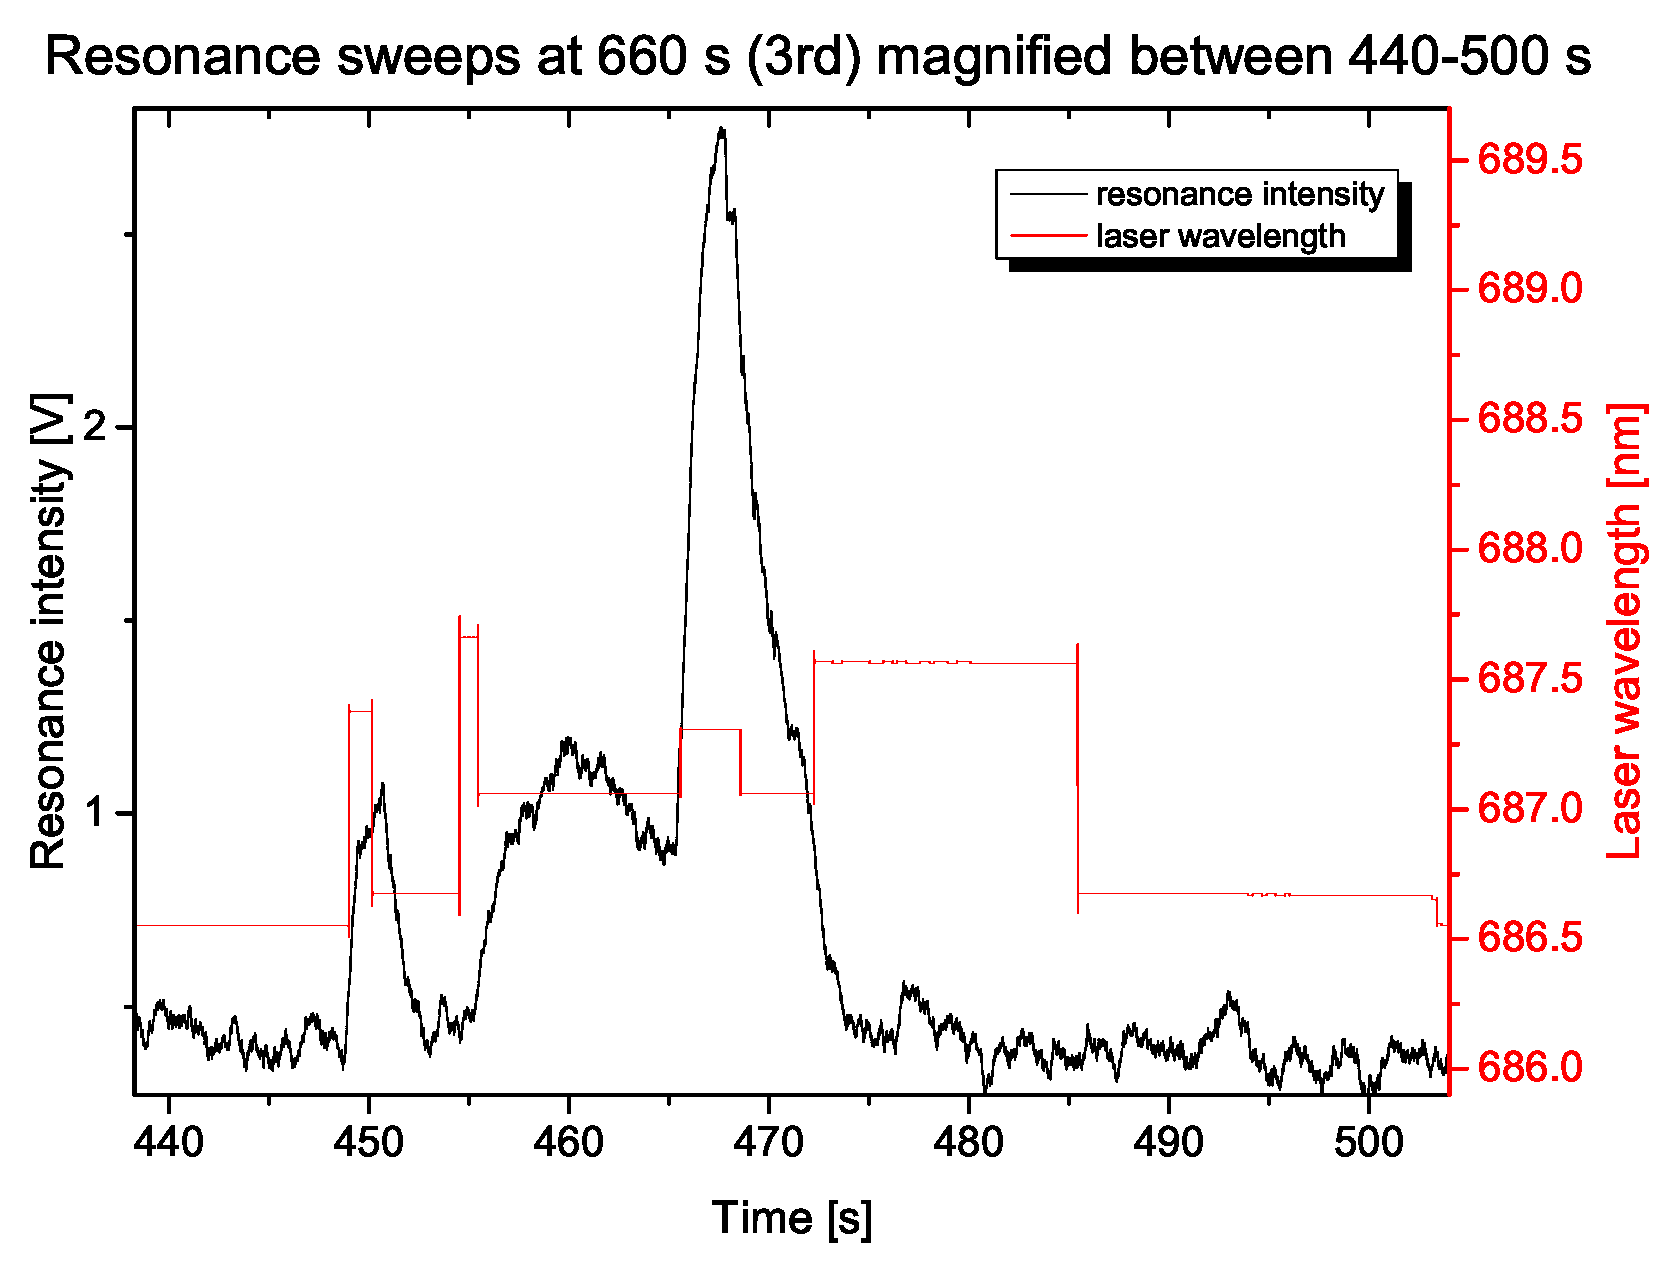
\includegraphics[width=\linewidth, height=10cm, draft=\foto]{eps/Graph10magnified.eps}}
\caption{In this measurement, the laser diode temperature is 0.1 $^\circ$C lower than \cref{primopicco}. We notice 3 different absorption wavelengths: 687.30, 687.35, 687.05 nm. Despite the laser jumps abruptly between the modes, the peaks look artificially continuous due to the low-pass filter in the lock-in amplifier.}\label{moltipicchi}
\end{figure} 

\medskip
Looking at the peak wavelength plots we noticed that the laser mode jumping is somehow periodical with respect to the piezoelectric sweeping voltage. That is, for portions of the sweep about 50-100 V large the modes hop from one to another according to a constant pattern.
This can be easily seen in \cref{hoppattern}, which shows both the wavelength of the main emission peak and his intensity of part of the sweep shown in \cref{fullsweep1}. The pattern, followed clearly for at least a couple of periods, is shown in \cref{tabrutta}.

\begin{figure}[!hbpt]\centering
\includegraphics[width=\linewidth, height=10cm, draft=\foto]{eps/periodicityofhops.eps}
\caption{We can see that the laser follows the same hopping pattern for several seconds, corresponding to a piezoelectric voltage sweep of 75 V.}
\label{hoppattern}
\end{figure}

\begin{table}[!hbpt]\centering
	\begin{tabular}{c|c}
		Time [s]&Wavelength [nm]\\
		\hline
		&687.50\\
		&686.60\\
		&687.40\\
		&687.70\\
		&687.05\\
		&687.30\\
		&687.05\\
		&687.55\\
		&687.00\\
		\hline
	\end{tabular}
\caption{Example of hopping pattern.}
\label{tabrutta}
\end{table}

DA QUI[
The laser diode features this periodicity not only with respect to the piezoelectric sweep, but is also noticeable observing of the uncontrolled frequency evolution (tm). 
Analysing more in detail this mode periodicity allowed also to see that different hops to the same mode do not hop exactly at the same frequency. While this periodicity imperfection usually only increased or decreased the part of the peak we were able to see, sometime it allowed us to scan during different measurements, different parts of the same peak therefore virtually enhancing the "tunability" range of the laser. ]A QUI. WTF DID I JUST READ?
% (scrivere di come in effetti sto aumento virtuale non sia quasi mai stato possibile da misurare a causa deella deformaz dei picchi dovuti alle instabilità o al semplice fatto che la nuova parte visibile è irrilevante (non contiene picco). 
 
		\subsection{Multiple full sweeps}
Since these measurement took quite a long time every sweep, doing repeated measurements most of time resulted in unmatchable data, because of the uncontrolled evolution we already mentioned. The influence of such uncontrolled factors exhibited however a random behaviour, so that, after some trials, we were able to get a unique \textquotedblleft lucky\textquotedblright measurement of 3 subsequent sweeps which matched almost perfectly. This is shown in \cref{3sweep}.

All the other attempts, however, resulted in severe changes of the resonance pattern between one sweep and another. Studying the pattern of the wavelength vs voltage graphic helps in realizing that this difference is not to be ascribed to the photoacoustic part of the experiment (oxygen concentration/pressure, laser alignment) but is rather due to a change in the laser emission wavelength pattern. \cref{3missweep,7sweeps} provide meaningful examples of this behaviour.
The change in the wavelength pattern is better shown in \cref{focus}, where we will focus
on shorter multiple sweeps around a single absorption peak.
\begin{landscape}
\begin{figure}[!bhtp]\centering
\includegraphics[height=\textheight, draft=\foto]{eps/3sweepsmatching.eps}
\caption{Three subsequent 0-150 V sweeps, of duration of 11 minutes each. Red: acoustic signal magnitude vs time and actuators voltage. Green: time projection. Blue: voltage projection. Notice that in the voltage projection the matching between the peaks of different sweeps in almost perfect. Laser parameters: 29,50 $^\circ$C; 80,01 mA.}
\label{3sweep}
\end{figure}\vfill
\end{landscape}

\begin{landscape}
\begin{figure}[!bhtp]\centering
\includegraphics[height=\textheight, draft=\foto]{eps/3mismatching.eps}
\caption{Despite these measurements are taken faster then usual (5 minutes each 0-150 V sweep) there is a big mismatch between the three sweeps. This mismatch is more evident in the magnitude vs voltage projection, where the peaks seem to be double-peaks. The time projections shows instead that they are
single peaks. Laser parameters: 27,68\cel; 80,01 mA}
\label{3missweep}
\end{figure}\vfill
\end{landscape}

\begin{landscape}
\begin{figure}[!bhtp]\centering
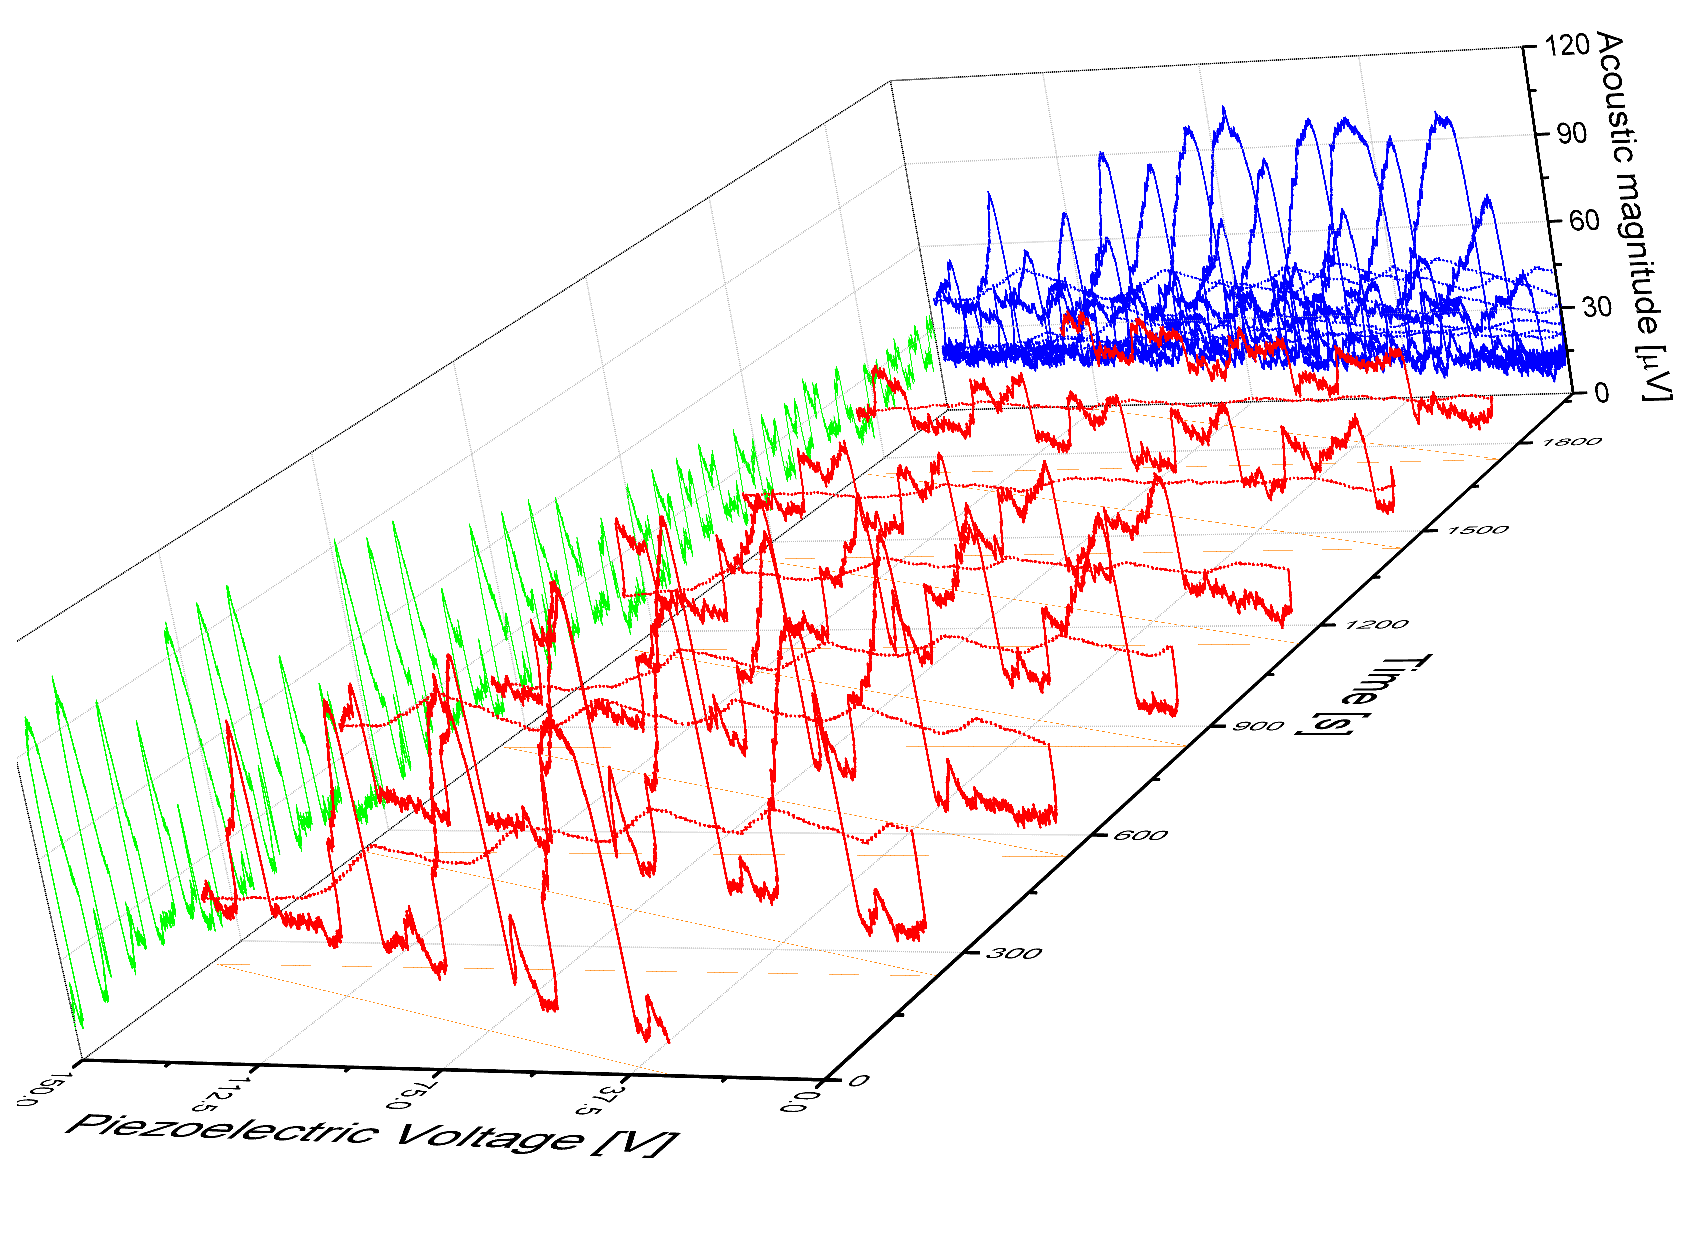
\includegraphics[height=\textheight, draft=\foto]{eps/7sweeps.eps}
\caption{In this measurement it is shown not only the fact that the peaks shift in voltage with time but can completely fade away after some minutes. Laser parameters: 25,03\cel; 80,01 mA}
\label{7sweeps}
\end{figure}\vfill
\end{landscape}
  
		\subsection{Multiple focused sweeps}\label{focus}
Another measurement methodology we used exploited repeated single-peak sweeps instead of 
full 0 to 150 V. This was intended to better study both the absorption peak shape and the evolution caused by external factors. In this kind of measurements it is also possible to use uncontrolled evolution at our advantage, since sometimes it allowed to increase the tunability range before a mode hopping. \cref{multisweep} shows how repeating a measurement of the same peak changed the part of the peak we were able to see. In \cref{multisweep1} the part of the peak we were able to see decreased after each sweep, while in \cref{multisweep2} the scanned part of the peak instead increased \textquotedblleft thanks\textquotedblright to the uncontrolled time evolution.
In both of these examples we see that we could not usually measure the "tunability range" using the spectrometer data, but still we are able to see that 
the voltage to laser mode dependence/pattern changes with time. 

\begin{figure}[!phtb]\centering
\subfigure[Laser parameters: 27,68\cel; 80,01 mA\label{multisweep1}]{\includegraphics[width=\linewidth, height=10cm, draft=\foto]{eps/multisweeps1.eps}}
\subfigure[Laser parameters: 25.03\cel; 80,01 mA\label{multisweep2}]{\includegraphics[width=\linewidth, height=10cm, draft=\foto]{eps/multisweeps2.eps}}
\caption{The resonance frequency shifts after every measurement, changing the part of the peak (in black) we were able to scan and decreasing the maximum measurable intensity.}
\label{multisweep}
\end{figure}

In order to better study how the voltage to wavelength output changed with time we plotted all the sweeps of \cref{multisweep1} on a voltage/intensity graphic, thus getting \cref{nonshiftedpeaks}, and subsequently shifted them by the voltage required to match the part of the peak which most likely corrisponded to the oxygen absorption peak (see \cref{factorsinfluencingtheshapeofthepeaks}), getting \cref{shiftedpeaks} as result.

\begin{figure}
\subfigure[\label{nonshiftedpeaks}]{\includegraphics[width=\linewidth, height=10cm, draft=\foto]{eps/multiunmatched.eps}}
\subfigure[\label{shiftedpeaks}]{\includegraphics[width=\linewidth, height=10cm, draft=\foto]{eps/multiunmatched.eps}}
\caption{}
\label{grafishifti}
\end{figure}

In order to make the edges of the peak match, we had to shift the various peaks of the values listed in the next table
\begin{table}[!htbp]
\begin{tabular}{|c|c|c|}
\hline
N of peak & Shift [V] & Delta Shift [V] \\ \hline
2 & -0.04 & -0.04 \\ \hline
3 & -0.065 & -0.025 \\ \hline
4 & -0.1 & -0.035 \\ \hline
5 & -0.12 & -0.02 \\ \hline
6 & -0.142 & -0.022 \\ \hline
7 & -0.157 & -0.015 \\ \hline
8 & -0.185 & -0.028 \\ \hline
9 & -0.195 & -0.01 \\ \hline
10 & -0.22 & -0.025 \\ \hline
\end{tabular}
\caption{Shifts of peaks in grafico /ref with respect to the first peak and to the precedent peak}
\label{peakshifts}
\end{table}

Wathing these graphics  and tables we could notice that the evolution is monotonic during our whole measurement, but his speed is not constant 
(every peak has to be shifted a different amount with respect to the quello prima).
GRAPHWAVELENGHTshifted
caption. In this graphic the wavelenght corresponding to each sweep has already been shifted of the same amount as the datain graph ref /shiftedpeaks
From the wavelenght/voltage graph we can also see that even after shifting the sweeps in order to make the edges of the peak match, the mode hopping from the 687.35nm 
mode (not corresponding to an absorption peak) and the 687.41 one is not matching between the various sweeps. This means that the "ambeintal evolution" is not 
correpsonding to a  simple "voltage drift" so that the voltage/wavelenght could be easily correctedby just a voltage shift, but has instead more complicated effects.
More efforts done to study the "evolution" are explained in the section /reflbldeqo.

/appendixinointerno?FACTORS INFLUENCING TEH SAHPE OF TEH PAKES.
tipregoqualcunoscrivaqualcuno.





---FREE LASER DRIFT----MAGARILOMETTODOPO[[  DA FAREEEEGEGEGEHEHE]]
NIGHT MEASURM
LONG MEASUREM
ETHALON MEASUREM

FOCUSED SINGLE PEAK SWEEPS
 
	\section{Laser shit (UNDER CONSTRUCTION)}
oiuyhgtfd

HERE IS MORE LASER SHIT
Because I am lorem ipsum
%%%%%%%%%%%%%%%%%%%
\begin{figure}[!htb]\centering
\vfill
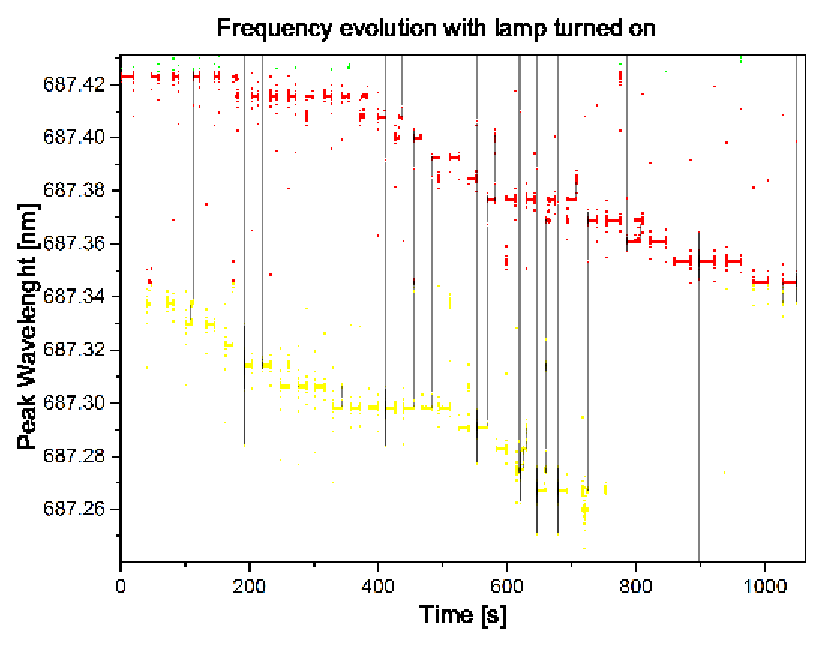
\includegraphics[width=\linewidth, draft=\foto]{eps/enlarged.eps}
\caption{THIS PICTURE IS A SHIT SHOT SHAT MADAFACCA}
\label{enged}
\end{figure}
%%%%%%%%%%%%%%%%%%%
so that in the shit that i go to the tiolet because unicorns eat chocolate and bloody kittens.
\begin{figure}[!htb]\centering
\includegraphics[width=\linewidth, draft=\foto]{eps/nighttime.eps}
\caption{furheuhfuhrueqpqpqpqpqp  dofwenofn EEE!}
\label{enorme}
\end{figure}

